\PassOptionsToPackage{margin=1in}{geometry}
\documentclass[12pt]{article}
\usepackage{wordlike} 
%\usepackage{mathptmx}
%\usepackage[scaled=.90]{helvet}
%\usepackage{courier}
\usepackage{graphicx}
\usepackage{float}
\usepackage{amsmath,amssymb,amsthm} % For including math equations, theorems, symbols, etc
\usepackage{subfig}
\usepackage{soul}
\graphicspath{{Figures/}} 
\usepackage{setspace}

\usepackage{hyperref}
\PassOptionsToPackage{dvipsnames}{xcolor}
\RequirePackage{xcolor} % [dvipsnames]
\definecolor{CTsemi}{gray}{0.55} % chapter numbers will be semi transparent .5 .55 .6 .0
\definecolor{CTcitation}{rgb}{0,0.5,0} % WebGreen
\definecolor{CTurl}{named}{Maroon} % Maroon
\definecolor{CTtitle}{named}{Maroon} % Maroon {cmyk}{0, 0.87, 0.68, 0.32}
\definecolor{CTlink}{named}{RoyalBlue} % RoyalBlue {cmyk}{1, 0.50, 0, 0}
\definecolor{halfgray}{gray}{0.55} % chapter numbers will be semi transparent .5 .55 .6 .0
\definecolor{webgreen}{rgb}{0,0.5,0}
\definecolor{webbrown}{rgb}{0.6,0,0}
\hypersetup{
	colorlinks=true,
	linkcolor=RoyalBlue,
	filecolor=magenta,      
	urlcolor=cyan,
	pdfkeywords={}
	breaklinks=true, bookmarks=true,bookmarksnumbered,
	urlcolor=webbrown, citecolor=webgreen, % Link colors
	pdftitle={}, % PDF title
	pdfauthor={\textcopyright}, % PDF Author
	pdfsubject={}, % PDF Subject
	pdfkeywords={}, % PDF Keywords
	pdfcreator={pdfLaTeX}, % PDF Creator
	pdfproducer={LaTeX with hyperref and ClassicThesis} % PDF producer
}


%opening
\title{Bayesian Evidence Synthesis:Opioid Crisis}
\author{Hyeongcheol Park*}

\begin{document}
%\renewcommand{\sectionmark}[1]{\markright{\spacedlowsmallcaps{#1}}}
 \maketitle{}
\tableofcontents % Print the table of contents
\listoffigures % Print the list of figures
\listoftables % Print the list of tables
\doublespacing

\section{Introduction}
The opioid crisis is a major issue in North America including British Columbia, Canada. British Columbia is in the midst of a drug overdose crisis due to illicit opioids and the circumstances are getting worse. According to the BC Coroners Service, there were more than 930 apparent illicit drug overdose deaths in BC from Jan. 1 to Dec. 31, 2016. This compares to 518 in 2015, an increase of 79.2\%. \cite{bccdc_opioid}  The goal of this project is to apply Bayesian evidence synthesis to better understand the opioid crisis in British Columbia, Canada.  \\ 

One difficulty in coping with the opioid crisis is that the total number of overdoses is unknown. The reason is that the use of prescription opioids often leads to use of illicit opioids and the extent of illicit usage cannot be known. Many of those who become addicted to opioids do so after initially receiving a prescription. The highly addictive nature of these pain relievers makes it easy for the human brain to crave more. It is only after their prescription ends that many users realize they’ve become dependent on the effects of opioids  to function “normally.” At that point, they are either forced to get clean and endure the pain that comes with the withdrawal symptoms of opioids or look for another means of getting their high. This is often the time where people will turn to illicit drugs or other analogues. Because prescription opioids are so expensive,  many users turn to heroin. It is often cheaper, more potent, and easier to locate than what they were taking before. In fact, about 80\% of people using heroin started with a prescription to another opioid. After using heroin, however, 23\% of individuals develop opioid addiction.\cite{opioid_desc} \\

Since the total number of overdoses is unknown, this number needs to be estimated. Bayesian statistics can be a way to approach the problem and give us a good estimate of the number with a defensible range of uncertainty. Bayesian statistics is a theory in the field of statistics based on the Bayesian interpretation of probability where probability expresses a degree of belief in an event. \cite{wiki_bayes} Further explanation is provided at the following section.\\


\section{Methods}

\normalsize 
The number of overdoses is our ultimate target of estimation. To achieve the goal in context of Bayesian statistics, we use our prior belief and available data set about the target of estimation. The posterior belief is coming from both of these sources of the information. Let $\theta$ denote all the unknown variables and let $Y$ denote all the related data sets. The following equation express the idea of Bayesian generative models in a mathmatical form:
\begin{equation}
\label{generic_bayes_thm}
\left.\begin{aligned}
p(\theta| Y ) = \frac{ p(\theta, Y)   }{ p(Y)} = \frac{ p(\theta) p(Y|\theta)}{ p(Y)} \propto p(\theta) p(Y| \theta), \end{aligned}\right.
\end{equation}

where $p(\cdot)$ is probability density (or mass) function. The equation \ref{generic_bayes_thm} states that the posterior belief of unobserved variables, $p(\theta|Y)$, is proportional to the mixture of the prior belief of the variables, $p(\theta)$, and the related data sets given the prior belief, $p(Y|\theta)$. Notice that the vector $\theta$ from equation \ref{generic_bayes_thm} includes parameters and latent variables, and hence it contains the total number of overdoses. \\

Let us assume that we are interested in the opioid crisis from month 1 to month T.  Let the subscript 1:T for any variable denote the variable for all target months and subscript t for any variable denote the variable of the month t. Then the target variable, the total number of overdoses from month 1 to month T  in British Columbia, is denoted by $O_{1:T}$.
\iffalse
Let $O_t$ denote the total number of overdoses in a given month $t$. 
\fi
In Bayesian concepts, the variable of interest $O_{1:T}$ is a vector of fixed numbers but the numbers are yielded from a certain distribution where the distribution describes knowledge about $O_{1:T}$; that is, each $O_t$ is considered to be a sample of a random variable. 
The simplest conceptual model is to take an underlying log-rate $z_t$ for each month $t$ where $z_t$ is independent and identically distributed across months according to a normal distribution with mean $\mu$ and variance $\sigma^2$. \cite{Irvine:modelling} Then let $\lambda_{t}^{OD}$ denote the rate of overdose at month $t$. It is assumed that the number of overdoses in the month, $O_t$, follows Poisson distribution with parameter $\lambda_{t}^{OD}N$ where the size of the population in the region of interest is $N$. Note that the population size, N, is unknown and vary over time in reality but it is assumed known and constant for the investigator here for simplicity. The mechanism is named as the overdose model  and is illustrated in mathmatical form below:

\iffalse
{The number of overdoses is our ultimate target of estimation. To achieve the goal in context of Bayesian statistics, we use our prior belief and available data set about the target of estimation. The posterior belief is coming from both of these sources of the information. The following equation express the idea in a mathmatical form:
\fi

\iffalse
\begin{equation}
\label{bayes_thm}
\left.\begin{aligned}
p(O_t| y ) = \frac{ p(O_t, y)   }{ p(y)} = \frac{ p(O_t) p(y| O_t)}{ p(y)} \propto p(O_t) p(y| O_t) \end{aligned}\right.
\end{equation}
\fi

\iffalse
where $O_t$ is the total number of overdoses in a given month $t$ in British Columbia, and $y$ represents the collected data set providing relevant samples of the target variable. In Bayesian concepts, the variable of interest $O_t$ is a fixed number but the number is yielded from a certain distribution where the distribution describes knowledge about $O_t$; That is, $O_t$ is considered to be a sample of a random variable. The problem, however, is that the data $y$ is not available. Hence it is needed to approach the estimation in an indirect fashion. 
\fi

\iffalse
 It is assumed that we are interested in the opioid crisis from month 1 to month T; subscript 1:T for any variable denotes the variable of every target months and subscription t denotes month t. The simplest conceptual model described in Figure \ref{simple_draw} is to take an underlying log-rate $z_t$ where that is independent and identically distributed across months according to a normal distribution with mean $\mu$ and variance $\sigma^2$. \cite{Irvine:modelling} Then let $\lambda_{t}^{OD}$ denote the rate of overdose at month $t$. It is assumed that the number of overdoses in the month, $O_t$, follows Poisson distribution with parameter $\lambda_{t}^{OD}N$ where the population of the region of interest is $N$. Note that the population size, N, is unknown and vary over time in reality but it is assumed known and constant for the investigator here for simplicity. 
\fi
 
 \begin{equation}
 \label{overdose}
 \left.\begin{aligned}
 z_{t} \sim N(\mu, \sigma^{2}), \\
 \lambda_{t}^{OD} = \exp(z_{t}),\\
 O_{t} \sim Poi(\lambda_{t}^{OD}N).
 \end{aligned}\right\} 
 \text{(overdose model)} 
 \end{equation}
 

 
Since estimation of $O_t$ is not straightforward as some of the variables ($\mu$, $\sigma$) determining $O_t$ is not known, we assume there was a survey conducted to help to support the inference about  $O_t$. The survey asked witnesses of opioid overdoses whether someone called an ambulance, for each month. This provides an estimate of the proportion of ambulance call $p_{A,t}$ among the overdoses. For the moment $p_{A,t}$ is assumed constant across time for simplicity. Let $n_{A,t}$ be the sample size of the survey at month $t$, and $x_{A,t}$ be the total number who confirmed that an ambulance was called at the month $t$. It is assumed that $x_{A,t}$ follows a Binomial distribution with number of trials, $n_{A,t}$, and  success probability for each trial, $p_{A,t}$. The mechanism is named as the ambulance call-outs model and is illustrated in mathmatical form below:

\begin{equation}
\label{ambulance}
\left.\begin{aligned}
x_{A,t} \sim Bin(n_{A,t},p_{A,t})\end{aligned}\right.
\text{(ambulance call-outs model).}
\end{equation}

Now the estimated $p_{A,t}$ can help to infer $O_t$ if there is a data regarding the number of  ambulance-attended overdoses. Let \(U_t\) be at a time point $t$. In general, the data of ambulance-attended overdoses \(U_t\) can be obtained. It is assumed that  \(U_t\) follows a Binomial distribution: 
\begin{equation}
\label{over_amb}
\left.
U_t \sim Bin(O_t, p_{A,t}).
\right.
\end{equation}

Note that $O_t$ can be estimated because $p_{A,t}$ can be infered from the survey data and the data regarding $U_t$ is given. Figure \ref{simple_draw} shows an example of how the estimation can proceed. The variables that can be observed (N, $U_{1:T}$, and $x_{A,1:T}$) are drawn in squares and the parameters ($\mu, \sigma^2$) and the latent variables ($\lambda_{1:T}, O_{1:T}, p_{A,1:T} $) that are not observarble from possible data sets are drawn in circles. Variables that need prior distributions are indicated with asterisks. The arrows indicate which variables affects which variables; for example, there is an arrow from $(\mu, \sigma^2)$ to $\lambda_{1:T}$ since $\mu, \sigma^2$ are the parameters of $\lambda_{1:T}$, and the two arrows from  $\lambda_{1:T}$ and $N$ to $O_{1:T}$ indicate that both $N$ and $\lambda_{1:T}$ affects the value of $O_{1:T}$ since the product of $\lambda_{1:T}$ and $N$ is the parameter of the distribution of $O_{1:T}$.\\

\begin{figure}[htb]
	\centering
	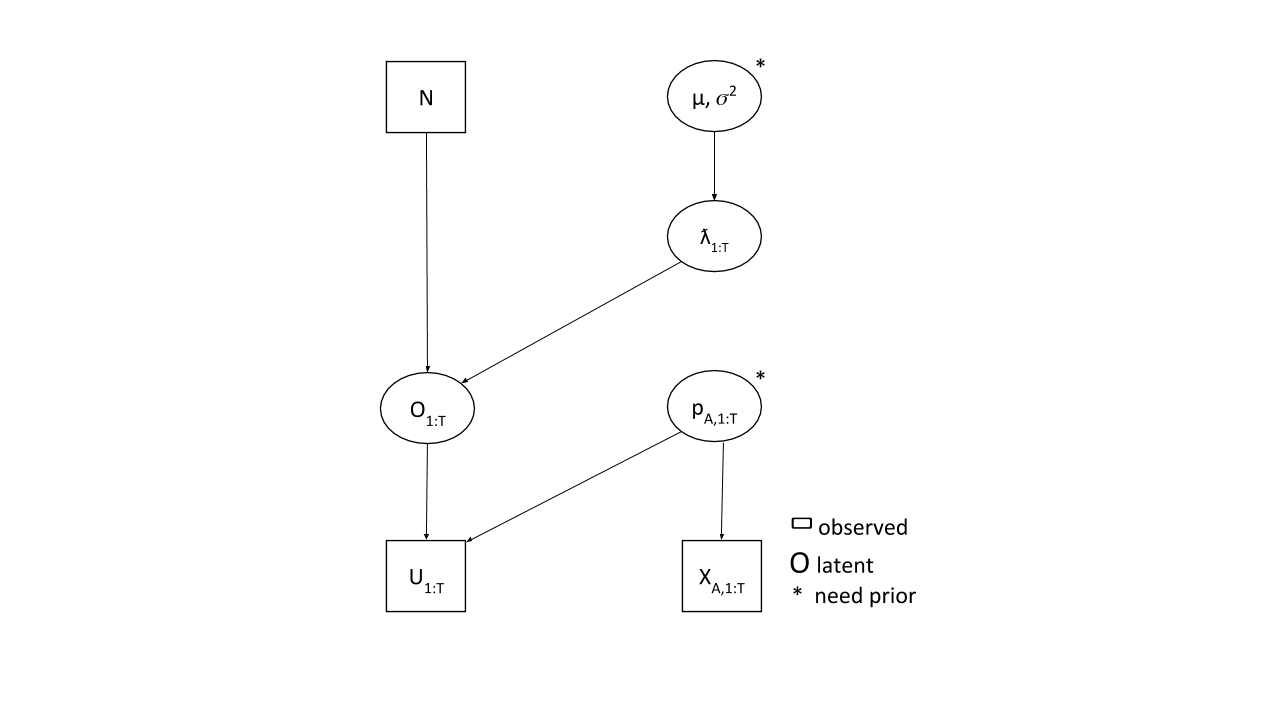
\includegraphics[width=200mm,scale=0.5]{Figures/simple_drawing}
	\caption[Example of estimating the total number of overdoses]{Example of estimating the total number of overdoses indirectly given two data sets: ambulance attended overdoses and survey data.}
	\label{simple_draw}
\end{figure}

We suggest a simple model in figure \ref{simple_draw} as a start where the model only combines Overdose Model \ref{overdose} and Ambulance Call-outs Model \ref{ambulance} with the relation \ref{over_amb}. The next step is to run some simulations to figure out how different types of inputs lead some changes of output.

\subsection{Generative Models}
The amalgamation of the prior distribution and the statistical model can be referred to as the generative model.\cite{paul} A generative model described in figure \ref{simple_draw} at a month $t$ can be written as follows given some a priori assumptions:

\begin{equation}
\label{gen_model}
\left.\begin{aligned}
p(\theta, Y) & =p(\mu,\sigma^2,\lambda_t, N, O_t, p_{(A,t)}, n_{(A,t)}, x_{(A,t)}, U_t) \\
& = p(\mu)p(\sigma^2|\mu)p(\lambda_t|\mu, \sigma^2)p(N)p(O_t|\lambda_t, N)p(p_{(A,t)})p(n_{(A,t)})p(x_{(A,t)}|p_{(A,t)},n_{(A,t)})p(U_t|O_t, p_{(A,t)}) \\
& \propto p(\mu)p(\sigma^2)p(\lambda_t|\mu, \sigma^2)p(O_t|\lambda_t, N)p(p_{(A,t)})p(x_{(A,t)}|p_{(A,t)},n_{(A,t)})p(U_t|O_t, p_{(A,t)}),
 \end{aligned}\right.
\end{equation}
where $\theta = (\mu, ,\sigma^2,\lambda_t, O_t, p_{(A,t)})$ and $ Y = ( N, n_{(A,t)}, x_{(A,t)}, U_t)$. The chain rule for random variables \cite{chain_rule} is used to the joint distribution of all variables at the first line of equation \ref{gen_model} such that the second line of the equation is derived.
A priori independence assumptions and conditional independence assumptions were presumed so that the second line of the equation is simplified. For example, it is asumed that  $\sigma^2$ and $\mu$ are independent to each other and $p_{A,t}$ and also all the variables from overdose model \ref{overdose}, ($\mu, \sigma^2, \lambda_t, N, O_t$), are independent to each other. 
Note that as a function of unknown variables, the function from the second line of the equation \ref{gen_model} is proportional to the function from the third line of the equation since $N$ and $n_{(A,t)}$ are presumed to be known and constants such that the density functions of the known variables are merely constants. Therefore the third line of the equation is the ultimate generative model of interest.\\

Conceptunally, generative model yields the posterior distribution $p(\theta|Y)$ on auto pilot since there exists only one distribution of $\theta$ given $Y$. we can use the distribution to make any inference claims that we need to make about parameters or latent variables such as point estimation and credibal interval.\\


\subsection{Simulation}

\normalsize 
Simulation can be used to predict the performance of the Bayesian models. In order to measure the performance of the simplified model, a data set was simulated and the process is described in this section. 

\subsubsection{Likelihood}

\normalsize 
There exist two data sets: the survey data ($n_{A,1:T}, x_{A,1:T}$), and the ambulance attended overdose data ($U_{1:T}$). The two data sets were simulated as follows. It was assumed that the two data sets were collected for a year (T=12). In terms of the survey data, it is assumed that  we have 12 survey data sets where each survey data set was collected for each month . The true value of $p_{A,t}$ was set as $p_{A,t}=0.8$ and the survey sample size $n_{A,t}$ was set as $n_{A,t}=1000$ for every month (t=1:T). The $x_{A,t}$ values for each month were independentally generated from the Binomial distribution (\ref{ambulance}).  
In terms of the overdose data, it is assumed that the total population size was $N = 10000$, and the true values of parameters for the overdose model were $\mu=\log0.05,\ \sigma=1$.
The vector of $O_t$ was generated following the overdose model (\ref{overdose}). The vector of $U_t$ was generated from the Binomial relation of the two variables ($\ref{over_amb}$). The two generated vectors have the same length as the survey data (T=12).  Note that only $U_t$ and $x_{A,t}$ are observable in the real-world application and $p_{A,t}$ needs to be estimated first in order to estimate $O_t$ which is the ultimate interest of the research.\\


\subsubsection{Prior Distributions}
\normalsize Noninformative prior distributions are presumed as a start for simplicity. 

\begin{equation}
\label{nonin_prior_amb}
p(p_{A,t}) \sim Beta(1,1)
\text{			noninformative prior for ambulance model}
\end{equation} 

\begin{equation}
\label{noninprior_over}
\left.\begin{aligned}
\mu \sim U(-10,0)\\
\sigma \sim U(0,5)
\end{aligned}\right\} 
\text{			noninformative prior for overdose model}
\end{equation}

This leads the posterior distribution of variables of interest to heavily depend on the likelihood. Later, the noninformative priors will be changed and the impact of the changes to posteriors will be investigated. 

\subsubsection{Markov Chain Monte Carlo}

The posterior distribution of the unseen variables-parameters ($\mu, \sigma^2, p_{A,1:T}$) and the latent variables ($\lambda_{1:T}, O_{1:T}$) given the seen variables, $Y$=($N, n_{(A,1:T)} x_{(A,1:T)}, U_{1:T}$), is the key to make any inference for any of the unseen variables $\theta$. For the inference about the variable of interest $O_{1:T}$, the marginal posterior distribution $p(O_{1:T}|Y)$ is essential which can be obtained by integrating the joint posterior distribution $p(\theta|Y)$ over all the other unseen variables except $O_{1:T}$. However, in general it is severely complicated and almost impossible to perform such multiple integrations because $p(\theta|Y)$ is a complex distribution of high dimension. Moreover, $p(O_{1:T}|Y)$ may not have closed-form nor follow a known parametric distribution, which makes the general inference procedure laborious.\\ 
 
Markov Chain Monte Carlo (MCMC) is a detour to obtain posterior samples from $p(\theta|Y)$ without explicitly knowing the distribution.  A Markov chain is a stochastic model describing a sequence of possible events in which the probability of each event depends only on the state attained in the previous event. In continuous-time, it is known as a Markov process. \cite{markov} Monte Carlo refers to the way how the inference of the target distribution is proceeded. Assessing the properties of a target distribution by generating representative random values is a case of a Monte Carlo simulation and any simulation that samples a lot of random values from a distribution is called a Monte Carlo simulation. \cite{gill}. MCMC technique allows us to generate Monte Carlo realizations of samples $\theta_{(i)}$ which are dependent, with the distribution of each sample $p(\theta_{(i)})$ converging to $p(\theta|Y)$.\cite{paul}.

\paragraph{Algorithms}

Gibbs sampling is a type of Metropolis algorithm that is used in JAGS. The Metropolis algorithm is a specific type of Monte Carlo process. It generates a random walk such that each step in the walk is completely independent of the steps before the current position. The proposed next step has no dependence on where the walk has been before, and the decision to reject or accept the proposed step has no dependence on where the walk has been before. The Metropolis algorithm is an example of a MCMC process. \cite{doing_bayes} \\

The No-U-Turn Sampler (NUTS) is a Hamiltonian Monte Carlo (HMC) Method that is used in pyMC3. HMC is a MCMC algorithm that avoids the random walk behavior and sensitivity to correlated parameters that plague many MCMC methods by taking a series of steps informed by first-order gradient information. These features allow it to converge to high-dimensional target distributions much more quickly than simpler methods such as random walk Metropolis or Gibbs sampling. However HMC’s performance is highly sensitive to two user-specified parameters: a step size and a desired number of steps. \cite{hoffman2011nouturn} Moreover, NUTS struggles to samples discrete random variables and hence it is recommended to approximate discrete random variables to continuous ones. The Poisson distribution from \ref{overdose} was approximated to Gamma distribution with the same parameter ($\lambda_{t}^{OD}N$) in pyMC3.

\paragraph{Assessing Convergence}

While independent samples of $\theta$ from the posterior distribution $p(\theta|Y)$ is of interest for any inference purpose, samples of $\theta_{(i)}$ generated by MCMC technique are (1), dependent samples and (2), the distribution of each sample $p(\theta_{(i)})$ are not exactly but only converges to $p(\theta|Y)$. It is essential to measure how well Monte Carlo realizations of samples approximate to the possible samples from the independent and identical posterior distribution. There are a few steps to examine the level of convergence.\\

First, it is mandatory to throw away some initial samples of Markov Chain realizations. Note that a value of $\theta_{(i)}$  from a lot of iteration better represents a sample from the posterior distribuion than some $\theta_{(j)}$ value from some early period of iterations ($i > j$). Since the convergence takes enough number of iterations, it is necessary to discard a chunk of the iterations from $\theta_{(1)}$ to $\theta_{(n)}$ for a large number $n$ enough to obtain the proper samples to represent the samples of interest from the posterior distribution. The period of iterations to be discarded is called burn-in period.
\\

Secondly, it is strongly recommended to have multiple starting points to assure the convergence. A visual way to check the convergence is to see a plot of  iteration numbers in x axis and their values for each iteration in y axis (trace plot). Note that $p(\theta_{(i)})$ converges to  $p(\theta|Y)$ regardless of the initial position of $\theta_{(1)}$, but the location of a initial position affects the number of iterations of MCMC algorithm for the convergence. Looking at only a single chain of iterations and their values may mislead us to believe that the number of iterations is enough while the trace of the values are staying at a local area before it reaches to the target distribution. By having more than one initial points and checking that the chains get mixed well and are stationary at a certain iteration point, we can verify that the algorithm reaches the desirable target distribution. 
\\

Lastly, numerical measures such as $\hat{R}$ and effective sample size can help us to examine the degree of convergence as well as looking at the trace plot of multiple chains of iterations. $\hat{R}$ is a measure of convergence where values for $\hat{R}$ near 1 suggest convergence. Effective sample size is a crude measure of the number of independent (effective) sample size from the total number of samples generated from a certain Markov chain. Both criteria is accessible after a generative model is fitted from a summary report of MCMC packages. The values of $\hat{R}$ and effective sample size in this report are obtainaed from JAGS. \\


\subsection{Initial Result} 

The achievement of the simulation was done by Markov chain Monte Carlo (MCMC). All examples here were performed in Python 3.8 with the library pyMC3 \cite{pymc3} and also in R 3.6.2 \cite{r_lan} with the JAGS 4.3.0 \cite{jags} library. All visualizations were the results from Python and pyMC3. Fitting was performed on a GHz Intel Core i5 with 8GM of LPDD3 RAM and typically had wall times under ten minutes. Code for all examples in this study are provided. 

\subsubsection{Posterior Distribution}


Figure \ref{pst_ot} is the boxplot of posterior samples of $O_t$. It is shown that our posterior estimates of  $O_t$ are fairly accurate since (1), the boxplots contain actual values of $O_t$ within their interquartile range (IQR), and (2), the ranges of IQR and 95\% range seem narrow. Notice that the range of the boxplot from a higher $O_t$ values (t=1, 7, 11) is wider than the other ranges of the boxplots from smaller estimates of $O_t$ (all t values but 1, 7, 11)\\

\begin{figure}[h]
	\centering
	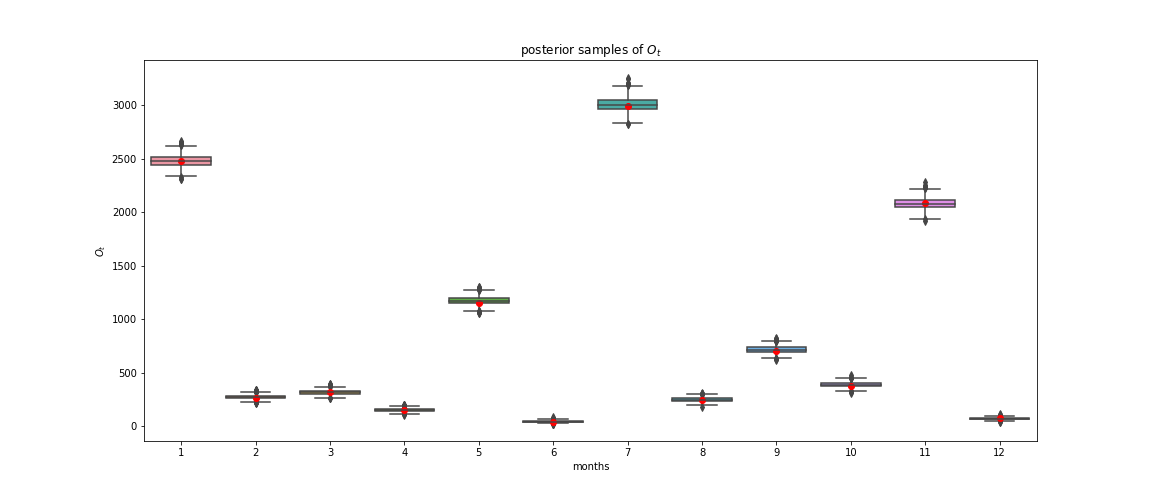
\includegraphics[width=1\linewidth]{Figures/earlyresult1_ot.png}
	\caption[Initial result: boxplot of posterior samples of $O_t$]{Boxplot of posterior samples of $O_t$ (2000 samples for each month) with simulated $O_t$ values as red dots.}
	\label{pst_ot}
\end{figure}

Let $O_+$ denote the total overdose per year ($O_+ = \sum_{t=1}^{12}O_t $). Figure \ref{hst_ot} is the histogram of posterior samples of the total number of overdoses $O_+$ per year. 3000 samples were collected and shown as the histogram.  It is seen that the plot is bell-shaped and not skewed. The 95\% credible interval of the total number of overdoses per year is between 10741 and 11164.\\

\begin{figure}[h]
	\centering
	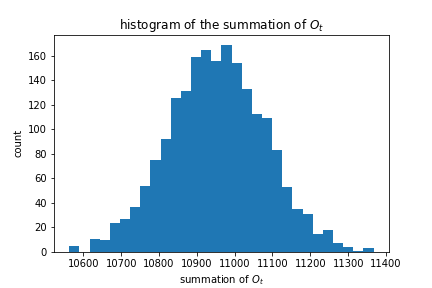
\includegraphics[width=1\linewidth]{Figures/hist_sum_ot.png}
	\caption[Initial result: histogram of posterior samples of total overdoses per year]{Histogram of posterior samples of total overdoses per year}
	\label{hst_ot}
\end{figure}

\newpage
\subsubsection{Posterior Predictive Check}
Posterior predictive checking is a model validation technique when we simulate some replicated data under the fitted model then compare the new data to the observed data. If the model fits, then replicated data generated under the model should look similar to observed data. To put it another way, the observed data should look plausible under the posterior predictive distribution. This is really a self-consistency check: an observed discrepancy can be due to model misfit or chance. \cite{bda_galman}\\

Figure \ref{ppc_ut} is the boxplot of posterior predictive samples of $U_t$. It is shown that the posterior predictive estimates of $U_t$ are failry accurate, for the same two reasons regarding the accuracy of the posterior distribution of $O_t$. It is more obvious here that the range of the boxplots from higher $O_t$ values (t=1, 7, 11) is wider than the other ranges of the boxplots from smaller estimates of $O_t$ (all t values but 1,7, 11). Notice that the relative ranges of figure \ref{ppc_ut} follow the ones of figure \ref{pst_ot}; for months where $U_t$ values are higher, the values of $O_t$ are also higher than the average (t=1, 7, 11).\\

\begin{figure}[htb]
	\centering
	\subfloat[ppc of $U_t$]{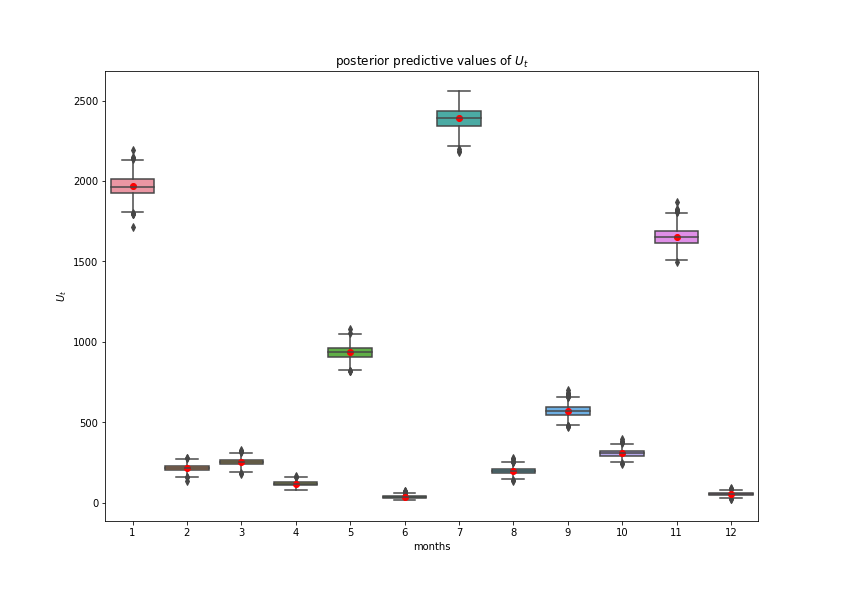
\includegraphics[width=.50\columnwidth]{Figures/early_r_ppc1_ut.png}\label{ppc_ut}}
	\subfloat[ppc of $x_{A,t}$]{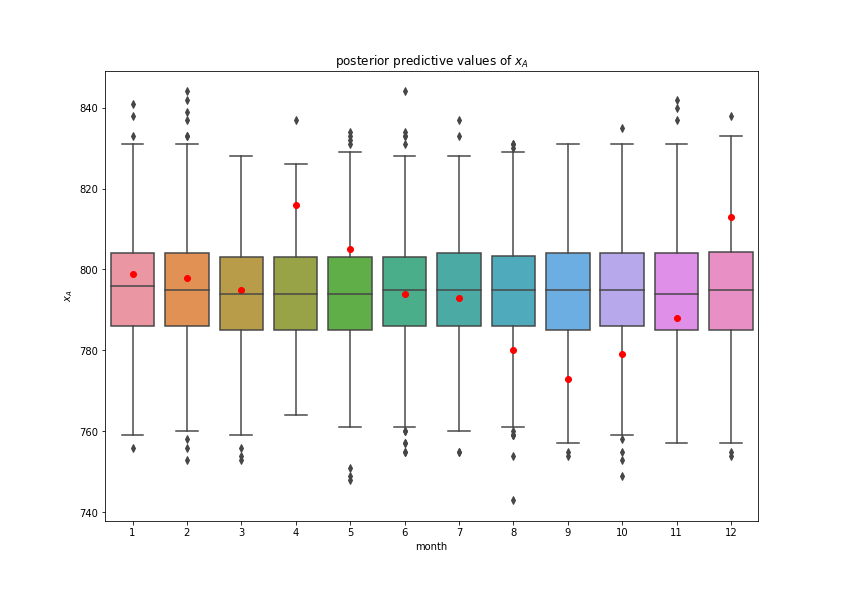
\includegraphics[width=.50\columnwidth]{early_r_ppc1_xt}\label{ppc_xt}}
	\caption[Initial result: box plots of predictive posterior samples of $U_t$ and $x_{A,t}$]{Boxplots of posterior predictive samples of $U_t$ and $x_{A,t}$ (1000 samples) with the actual data point of simulated $U_t$,$x_{A,t}$ value. The simulated values are shown as a red dots.}
	
\end{figure}

Figure \ref{ppc_xt} is the boxplots of posterior predictive samples of $x_{A,t}$. It is shown that the posterior predictive estimates of $x_{A,t}$ are tolerably accurate since (1), the boxplots contain actual values of $O_t$ within their lines connecting the maximum and the minimum, and (2), the ranges of IQR seem narrow. \\



\subsection{Result: Contamination of $p_{A,t}$ } 
One focus of this research project is to investigate how robust the model is to contaminations of the data sets. The first inspection is to check an impact of a contamination of $p_{A,t}$; what would happen if the estimation of $p_{A,t}$ is biased? It is assumed that the survey data gives us a wrong estimate of $p_{A,t}$ such that it would be underestimated or overestimated. We then want to see how the biased estimation of $p_{A,t}$ affects the estimate of $O_t$, the total number of overdoses.\\

Both underestimation and overestimation were considered for the analysis. In terms of underestimation, the simulated survey data ($n_{A,t}, x_{A,t}$) was generated with $p_{A,t}=0.6$ while the true value of $p_{A,t}$ is 0.8 for all $t$ ($t=1,2,3, ..., 12$), and all the other assumptions hold as before. That is, $x_{A,t}$ is generated from $x_{A,t} \sim Bin(n_{A,t}, 0.6)$, while $U_t$ is generated from $U_t \sim Bin(O_t, 0.8)$ for every $t$. For overestimation, the simulated survey data was generated with $p_{A,t}=0.9$ while the true value of $p_{A,t}$ is 0.8, and all the other assumptions hold the same.  \\

\subsubsection{Posterior Distribution}

\begin{figure}[htb]
	\centering
	\subfloat[ppc of $O_t$: underestimated $p_{A,t}$]{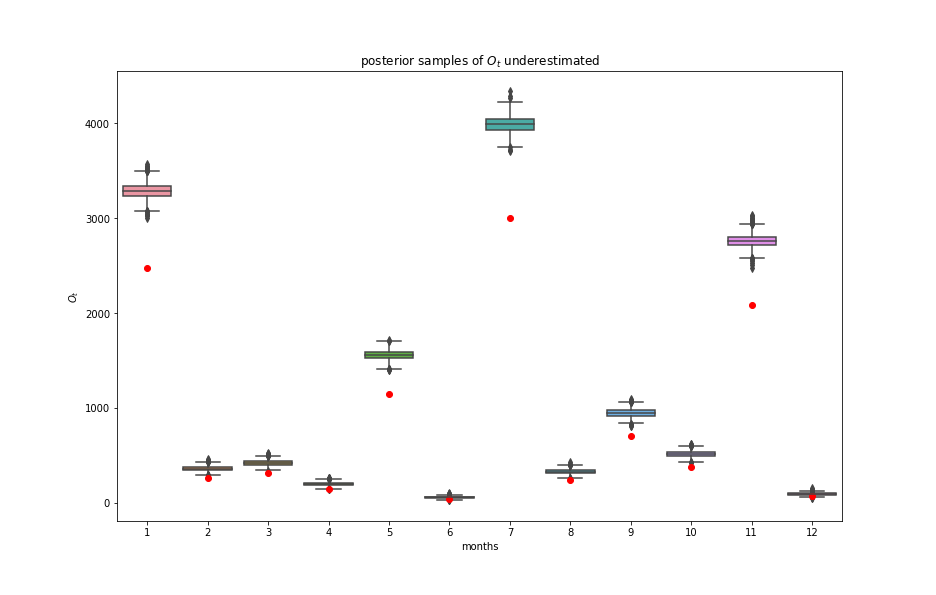
\includegraphics[width=.50\columnwidth]{early_contamination_underestimated-o_t.png}\label{under_ot}}
	\subfloat[ppc of $O_t$: overestimated $p_{A,t}$]{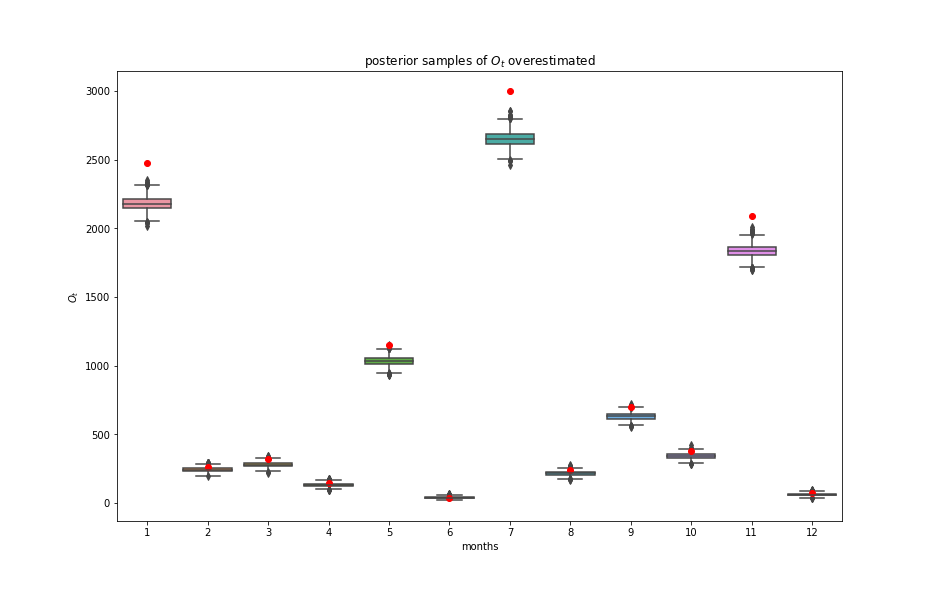
\includegraphics[width=.50\columnwidth]{early_contamination_overestimated-o_t}\label{over_ot}}
	\caption[Contaminated $p_{A,t}$: boxplot of posterior samples of $O_t$ ]{Boxplot of posterior samples of $O_t$ (1000 samples) where survey data is contaminated.  The actual data point of simulated $O_t$ values are shown as red dots.}
	\label{contam_ot}
\end{figure}

\normalsize 
Figure \ref{contam_ot} is the boxplots of posterior samples where $p_A$ is contaminated from the survey data. It is seen that the underestimation of $p_A$ (\ref{under_ot}) leads to an overestimation of $O_t$ as the boxplots are above the red dots. This is explainable considering the given data sets (likelihoods) and the relationship between the two models (\ref{over_amb}); given the likelihood of the ambulance attended overdoses, $U_t$, a value of $O_t$ is an unknown parameter of the binomial distribution, $Bin(O_t, p_A)$. Let $o_t$, $u_t$ denote posterior samples from $O_t$ and the observed value of $U_t$ respectively. Then $o_t$ is proportional to the quantity generated by multiplying $u_t$ and the inverse of $\hat{p}_{A}$ where $\hat{p}_{A}$ is underestimated estimator of $p_A$; hence $\frac{1}{\hat{p}_{A}}$ is overestimated which leads overestimation of $O_t$:
\begin{equation}
\label{ot.how.made}
\begin{aligned}
o_t \propto u_t \frac{1}{\hat{p}_{A}}.
\end{aligned}
\end{equation}
Figure \ref{over_ot} shows the opposite case. Overestimation of $p_A$ leads underestimation of the inverse of $p_A$ which causes underestimation of $O_t$. From both figures it is seen that the bias increases as the estimated values and the actual values get large.\\

\subsubsection{Posterior Predictive Check}

Figure \ref{contam_ut} gives the boxplots of posterior predictive samples where $p_{A,t}$ is underestimated and overestimated respectively from the survey data. It is seen that none of the contaminations of $p_{A,t}$ lead to an contamination effect on $U_t$ but only affect the $O_t$ estimation.\\

The possible explanation is that the contaminations of  $p_{A,t}$ and $O_t$ (from $p_{A,t}$) cancel out the bias component as combined so that $U_t$ has no bias. Notice that $U_t$ is a likelihood (data set) of $O_t$ estimation. Hence it plays the role of $Y$ in Bayes theorem (\ref{generic_bayes_thm}) and the likelihood, $U_t$, is used to obtain the biased posterior samples of $O_t$ with the contaminated estimates of $p_A$. Here the pair of $(O_t, P_{A,t})$ are both biased and the pair is fitted by the likelihood, $U_t$. To obtain the posterior predictive samples, MCMC algorithm help obtain posterior samples of biased $O_t$ and then the samples will be combined with biased $p_A$ such that the new samples of $\tilde{U_t}$ from $p(\tilde{U_t}|{U_t})$ is obtained.  The result also matches with our intution. Posterior predictive checks use the existing data points twice; firstly it uses the data to obtain the posterior samples of parameters, and secondly the samples are used to produce posterior predictive samples. Given the fact that there could be an overfitting issue due to using the data twice, the result shown here seems reasonable. 
\\

\begin{figure}[htb]
	\centering
	\subfloat[ppc of $U_t$: underestimated $p_{A,t}$]{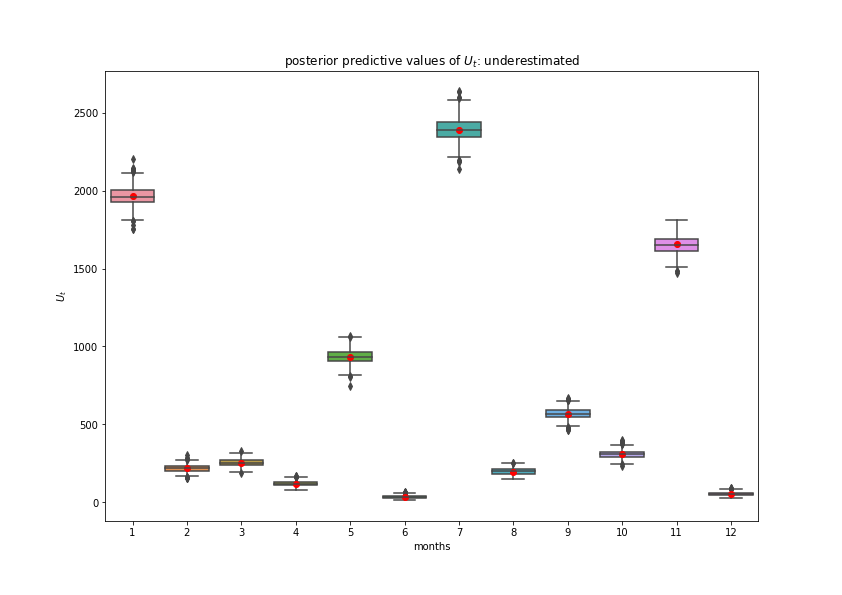
\includegraphics[width=.50\columnwidth]{early_contamination_underestimated-u_t.png}\label{under_ut}}
	\subfloat[ppc of $U_t$: overestimated $p_{A,t}$]{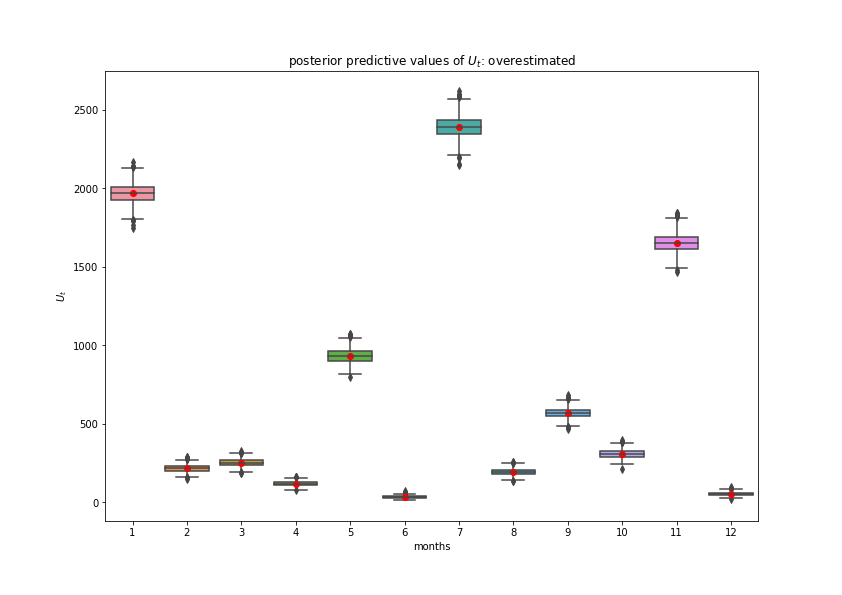
\includegraphics[width=.50\columnwidth]{early_contamination_overestimated-u_t}\label{over_ut}}
	\caption[Contaminated $p_{A,t}$: boxplot of posterior samples of $U_t$]{Box plot of posterior samples of $U_t$ (1000 samples) where survey data is contaminated.  The actual data point of simulated $U_t$ values are shown as red dots.}
	\label{contam_ut}
\end{figure}

Figure \ref{contam_xt}  gives the boxplots of posterior predictive samples of $x_{A,t}$ where $p_{A,t}$ is underestimated and overestimated respectively from the survey data. It is seen that none of the contaminations of $p_{A,t}$ leads an effect of contamination on $x_{A,t}$; the actual simulated points (red dots) are close to the medians from the two boxplots. However, notice that the range of the estimated values are different between the two boxplots; the median from Figure \ref{under_xa} is around 600 whereas the median from Figure \ref{over_xa} is around 900. This implies that the posterior predictive samples match the biased given data sets (with $p_{A,t}=0.6$ and $p_{A,t}=0.9$ respectively) but the samples cannot estimate the unbiased true value of $p_{A,t}$, which is 0.8. This is because overdose model (\ref{overdose}) does not affect the result from the ambulance model (\ref{ambulance}); only the ambulance model has an effect on the overdose model as it is seen from figure \ref{simple_draw}.

\begin{figure}[h]
	\centering
	\subfloat[ppc of $x_{A,t}$: underestimated $p_{A,t}$]{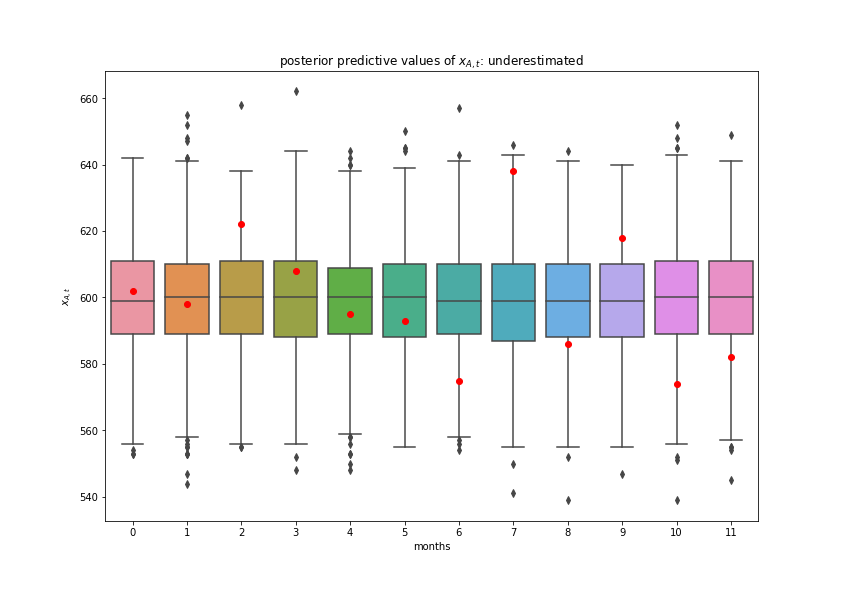
\includegraphics[width=.50\columnwidth]{early_contamination_underestimated-x_a.png}\label{under_xa}}
	\subfloat[ppc of $x_{A,t}$: overestimated $p_{A,t}$]{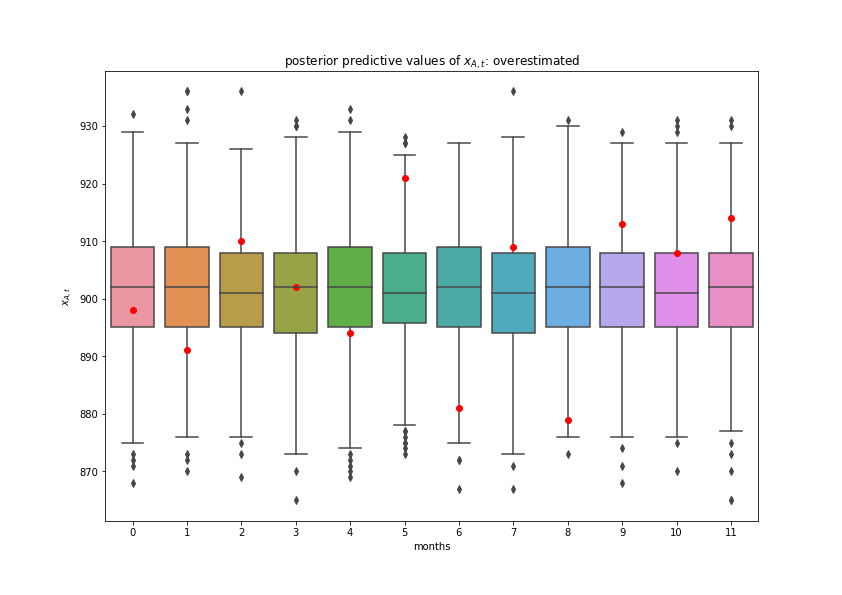
\includegraphics[width=.50\columnwidth]{early_contamination_overestimated-x_a.png}\label{over_xa}}
	\caption[Contaminated $p_{A,t}$:: boxplot of posterior samples of $x_{A,t}$]{Boxplot of posterior samples of $x_{A,t}$ (1000 samples) where survey data is contaminated.  The actual data point of simulated $x_{A,t}$ values are shown as red dots.}
	\label{contam_xt}
\end{figure}

\subsection{Result: Unobservable $N$}
In practice, it is reasonable to assume that investigators only have a general idea about the total population size of the reigion rather that they know the exact value of the total population size. The assumption of the known value of the total population size for a region, $N$, from the previous section changes to be unknown in this section to see the impact of the likelihood over the posterior distributions of variables of interest. The generative model at a month $t$ can be written as follows given some a priori assumptions:

\begin{equation}
\label{gen_model_unk_N}
\left.\begin{aligned}
p(\theta, Y) & =p(\mu,\sigma^2,\lambda_t, N, O_t, p_{(A,t)}, n_{(A,t)}, x_{(A,t)}, U_t) \\
& = p(\mu)p(\sigma^2|\mu)p(\lambda_t|\mu, \sigma^2)p(N)p(O_t|\lambda_t, N)p(p_{(A,t)})p(n_{(A,t)})p(x_{(A,t)}|p_{(A,t)},n_{(A,t)})p(U_t|O_t, p_{(A,t)}) \\
& \propto p(\mu)p(\sigma^2)p(\lambda_t|\mu, \sigma^2)p(N)p(O_t|\lambda_t, N)p(p_{(A,t)})p(x_{(A,t)}|p_{(A,t)},n_{(A,t)})p(U_t|O_t, p_{(A,t)}),
\end{aligned}\right.
\end{equation}

where $\theta = (\mu, ,\sigma^2,\lambda_t, O_t, p_{(A,t)}, N)$ and $ Y = (n_{(A,t)}, x_{(A,t)}, U_t)$. Notice that $N$ is an element of $\theta$ instead of an element of $Y$ and the model contains a prior distribution of $N$. The chain rule for random variables \cite{chain_rule} is used to the joint distribution of all variables at the first line of equation \ref{gen_model_unk_N} such that the second line of the equation is derived.
A priori independence assumptions and conditional independence assumptions were presumed so that the second line of the equation is simplified. The model is shown graphically in figure \ref{draw_N} where $N$ is a latent variable with a prior distribution needed.\\

\begin{figure}[htb]
	\centering
	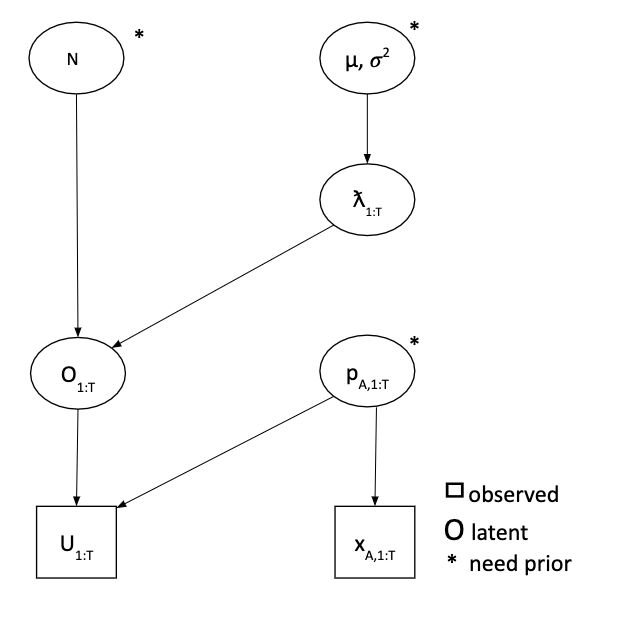
\includegraphics[width=100mm,scale=0.3]{Figures/draw_N}
	\caption{Generative model with unoberservable $N$}
	\label{draw_N}
\end{figure}

Suppose we have some information about the population size such that we transform it into a prior distribution; the prior distribution of $N$ should reflect our prior knowledge about $N$ which we have even before we encounter the data set. As a start,  $N$ is assumed to follow symmetric prior distribution: 

\begin{equation}
\label{in_prior_N}
N \sim Normal(10000,1000)
\text{ (informative prior for the total population size),}
\end{equation} 

where the prior information suggests that $N$ is most likely around 10000 and $\pm 20\%$ of the point estimation covers  95\% of the symmetric support of $N$.
\subsubsection{Posterior Distribution}
Both MCMC algorithms from pyMC3 and JAGS suffered from relatievely long running time of the algorithms and the convergence issue of the trace of $N$. The reason of having the stationarity issue is that too much inference has been asked to the data sets. Only two data sets, $U_{1:T}$ and $(n_{A,1:T}, x_{A,1:T})$, are given and the task was to generate posterior samples of 5 random variables, $N, \mu, \sigma^2, \lambda_{1:T}, O_{1:T}, p_{A,1:T}$. Figure \ref{trace_N} shows the trace plot and the posterior density plot of $N$. From the trace plot of $N$ it is seen that the chains are mixed well but not stationary and thus not convenging; two chains of the variable covered a common distribution but neither sequence appeared stable even after 10000000 iterations. The effective sample size for N was only 56271. The posterior distribution seems to be roughly symmetric at the center 10000. 
\begin{figure}[htb]
	\centering
	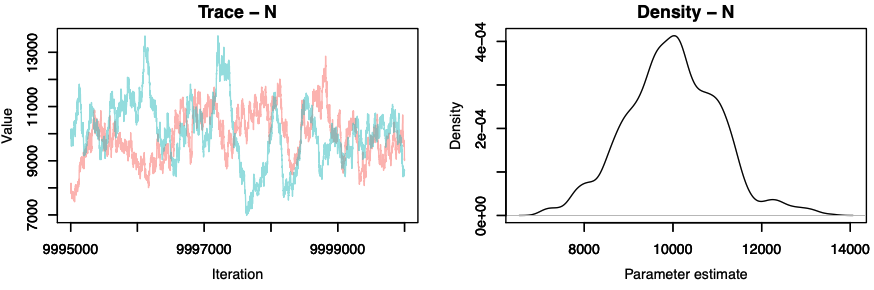
\includegraphics[width=1\linewidth]{Figures/not_mixed_N.png}
	\caption[Unobserved $N$: trace plot of latent variable $N$]{Trace plot of latent variable $N$}
	\label{trace_N}
\end{figure}

Figure \ref{hist_unk_n} shows the posterior samples of $N$. Due to the computational cost and the restriction of computing power of the research device, only 20000 samples were generated from the model. The plot reveals that the posterior distribution is centered around the true value, 10000, and symmetric around the center. The result is likely to be due to the prior distribution. The prior distribution was providing exact and accurate information about $N$ such that the posterior distribution remains the similar shape although there is a convergence issue. Further research is recommended to investigate the effect of prior distribution to the posteior distribution of $N$.	

\begin{figure}[htb]
	\centering
	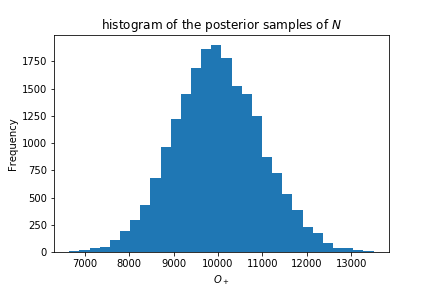
\includegraphics[width=0.7\linewidth]{Figures/hist_N.png}
	\caption[Unobserved $N$: boxplot of posterior samples of $N$]{Boxplot of posterior samples of $N$ (20000 samples for each month)}
	\label{hist_unk_n}
\end{figure}

Figure \ref{pst_ot_unk_n} shows that the inference of $O_{1:T}$ as accurate as before. This was possible as the proper prior distribution of $N$ yields acceptable estimation of $N$ which dominates the estimation of $O_t$ with $\mu, \sigma^2$ from figure \ref{draw_N}. Any distortion of the prior distribution of $N$ may affect the inference result of $O_{1:T}$.

\begin{figure}[htb]
	\centering
	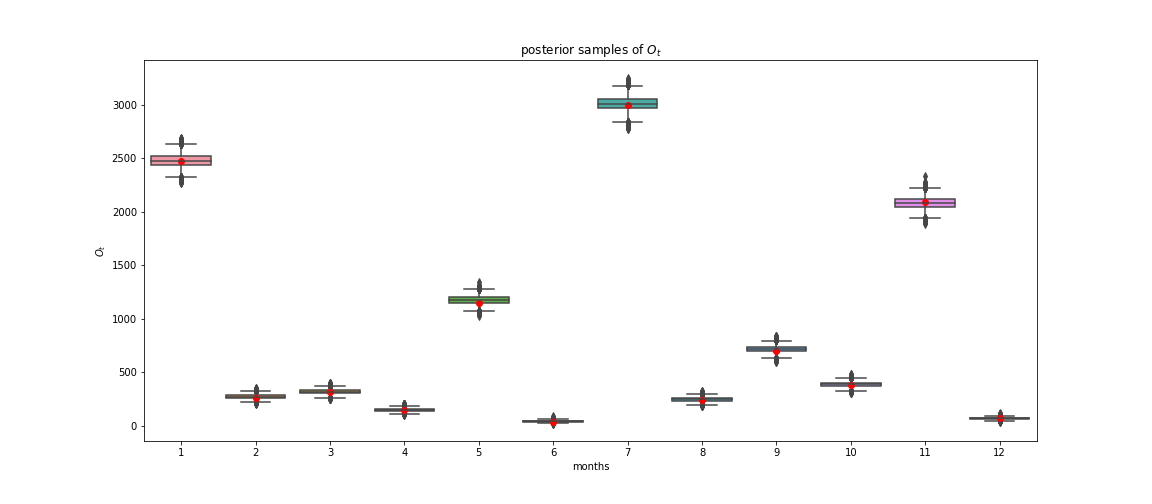
\includegraphics[width=1\linewidth]{Figures/unknown_N_ot.png}

	\caption[Unobserved $N$: boxplot of posterior samples of $O_t$]{Boxplot of posterior samples of $O_t$ (20000 samples for each month) with simulated $O_t$ values as red dots.}
	\label{pst_ot_unk_n}
\end{figure}

\subsubsection{Posterior Predictive Check}

Figure \ref{ppc_unk_n} is the boxplot of posterior predictive samples of $U_t$ and $x_{A,t}$. It is shown that the posterior predictive estimates of $U_t$ and $x_{A,t}$ are failry accurate for the same reason regarding the accuracy of the posterior distribution of $O_t$.

\begin{figure}[htb]
	\centering
	\subfloat[ppc of $U_t$]{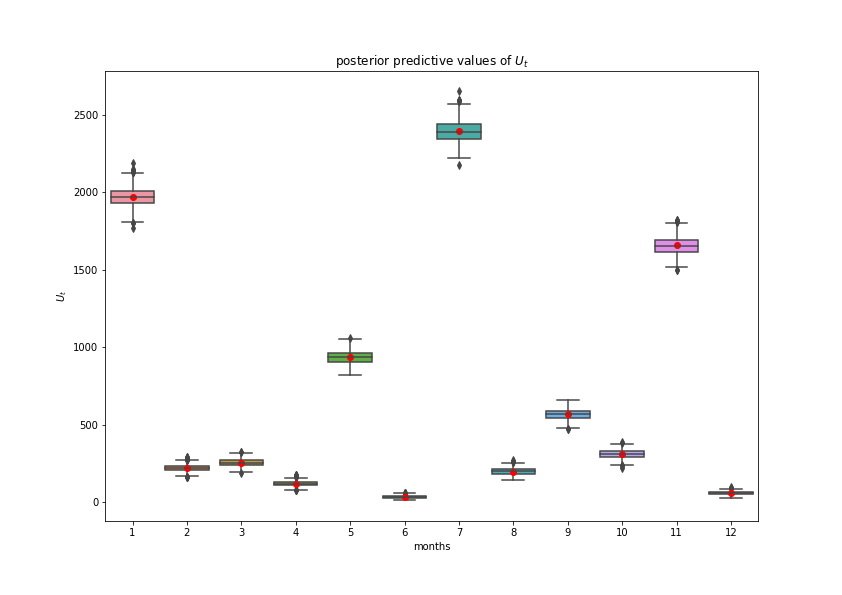
\includegraphics[width=.50\columnwidth]{Figures/unk_N_ppc1_ut.png}\label{ppc_ut_unk_n}}
	\subfloat[ppc of $x_{A,t}$]{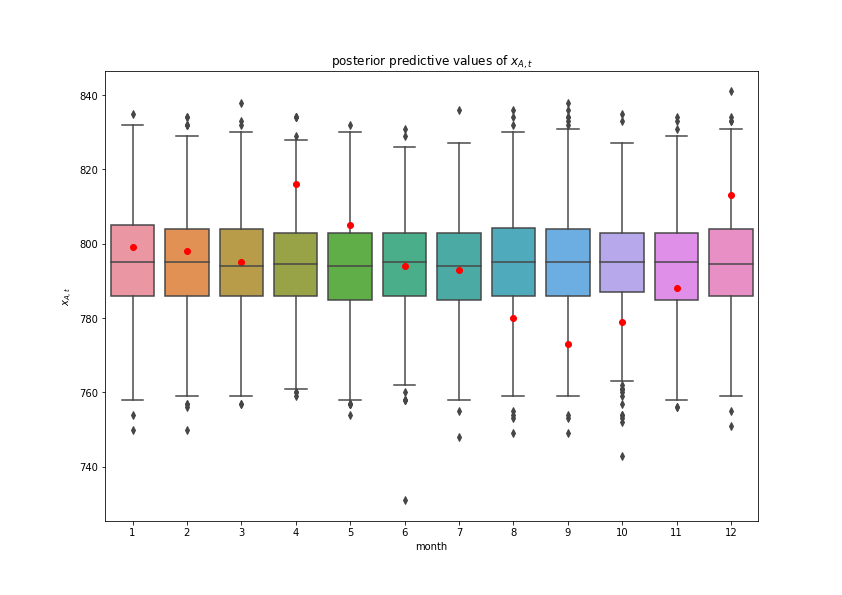
\includegraphics[width=.50\columnwidth]{unk_N_ppc1_xt}\label{ppc_xt_unk_n}}
	\caption[Unobserved $N$: box plots of predictive posterior samples of $U_t$ and $x_{A,t}$]{Boxplots of posterior predictive samples of $U_t$ and $x_{A,t}$ (1000 samples each) with the actual data point of simulated $U_t$, $x_{A,t}$ value. The simulated values are shown as a red dots.}
	\label{ppc_unk_n}
\end{figure}

\section{Conclusion}
 
Bayesian statistics and generative model is an outstanding approach for statistical inference which incorporate available data sets and our  prior knowlede and information. Bayesian model can cope with prior research outcomes as our prior information whereas frequentist approach cannot absorb the knowledge in their models. Furthermore, Bayesian modeling is intuitive to us since Bayesian viewpoint to probability corresponds to our conceptual perspective about probability. \\ 

However, Bayesian models have their own weaknesses. In cases where the problems are immensely complicated, the models suffer much more than the Frequentist models from long computational time of MCMC algorithms. This issue has been being relived as the general computing power of machines has been improved and decent MCMC algorithms have been developed to reduce waiting time although patient waiting is still a virtue to Bayesian statisticians.\\
 
Note that the robustness of models shoud be confirmed. If there exist some contaminations of data sets, the result of posterior estimations may not be trustworthy and therefore it is needed to confirm how robust the result of models is from the contaimiations. Likewise, it is generally recommended to apply more than one MCMC algorithms to the generative model to confirm that Monte Carlo realizations of  samples are robust to different types of the algorithms.\\
 
Lastly, notice that it is not reasonable to provide few data sets and ask Bayesian generative models to yield decent results; the models are not a god-like solver for every qnatitative problems. It is shown from the previous section that asking about the total population size $N$ is too much to ask for the model while the survey data $(n_{A,1:T}, x_{A,1:T})$ and the data of the number of ambulance-attended overdoses $(U_{1:T})$ are only provided.	\\

\bibliographystyle{alpha}
\bibliography{sample.bib}
\end{document}
